\chapter{Le contexte de résolution du problème}
\chaptermark{Contexte}
\minitoc
\newpage
 
\section{Introduction}

La matière première de Transaction Connect est la donnée de transaction que génèrent les clients en faisant les achats dans les magasins. Ces données brutes sont soumises à des traitements afin de ressortir d’autres informations  importantes notamment le centre commercial visité, et le magasin d’achat.

\begin{figure}[h]
\begin{center}
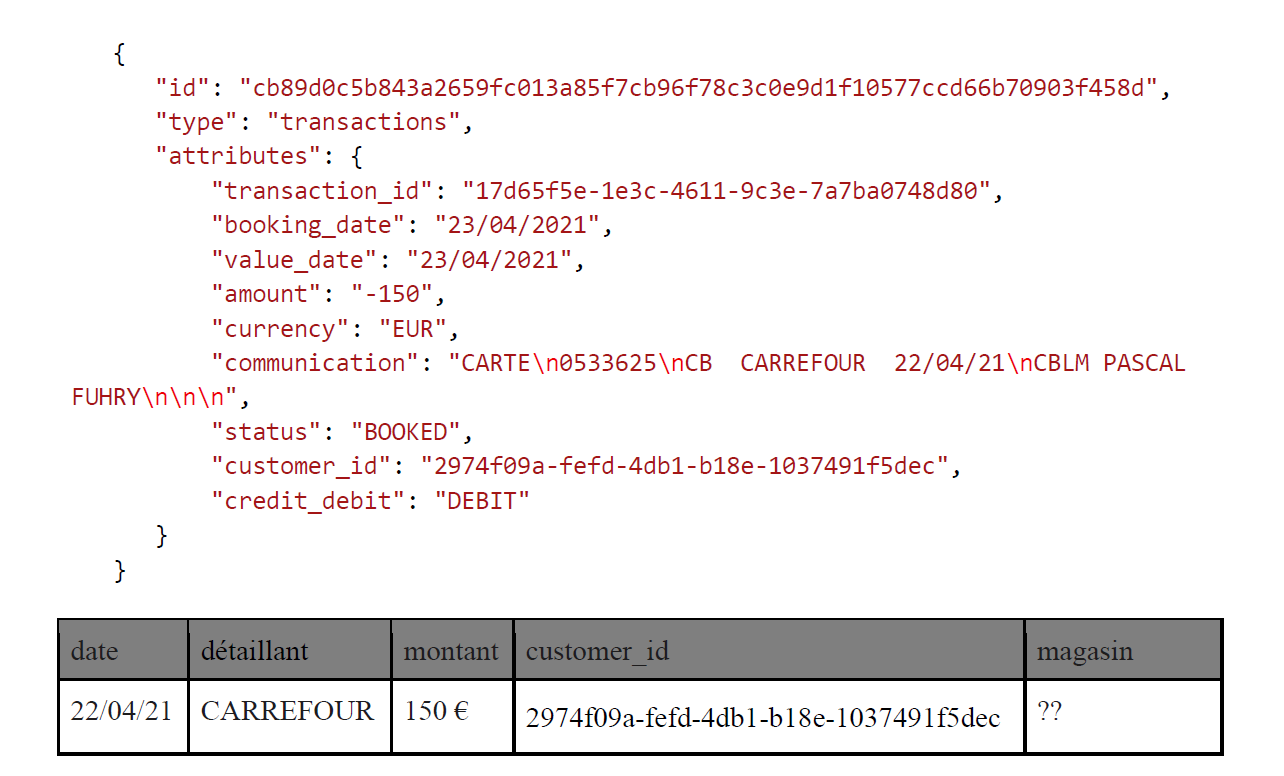
\includegraphics[width=15cm,height=9cm]{images/format_transac.png}
\caption[Exemple de transaction à enrichir}
\label{monlabel}
\end{center}
\end{figure}

Après avoir extrait les informations nécessaires, l’objectif maintenant est d’identifier l’origine de la transaction, le magasin de provenance de cette transaction. La réponse à cette question nous permet d’identifier si ce magasin fait partie du centre commercial où le client est fidélisé. Dans le cas affirmatif, le client gagne des points correspondant au programme de fidélité de ce Centre commercial.

\newpage
\section{Le problème à résoudre} 
En interne, il existe plusieurs méthodes d’affectation des transactions tant en machine learning que algorithmique. 
Les principaux algorithmes d’affectation des transactions:
\begin{itemize}
\item Le store locator
\item Alpha / Alpha City
\item Patterns regex
\item Le Scoring
\end{itemize}
Le problème à résoudre durant mon parcours en tant que stagiaire sera autour de la classification et l'affectation aux magasins des transactions en utilisant l’algorithme du scoring. Le scoring est le quatrième algorithme de Transaction Connect permettant l’affectation des transactions remontant avec moins d’informations dans les labels qui peuvent permettre l’identification de l’origine de transaction. C’est une méthode de machine learning basée sur la probabilité visant à analyser le comportement d’achat des clients dans une journée afin de retracer une transaction inconnue à partir d’autres transactions identifiables dans la même journée.
L’objectif final sera dans un premier temps d'améliorer la qualité d’affectation des transactions grâce au Scoring. 
Dans le but d’améliorer l’ancienne version du scoring, je serai amené à:
\begin{itemize}
\item Procéder au feature engineering en faisant la migration des requêtes de Postgresql vers Redshift dans le but de diminuer la durée des calculs.
\item Mettre en place des modèles de scoring spécifique d’affectation des transactions de certains grands centres commerciaux
\item Automatiser le choix du modèle idéal correspondant en se basant sur les métriques de test.
\item Automatiser la construction de nouveaux modèles en prenant en compte des données récentes sur une période mensuelle.
\end{itemize}

\section{Features engineering (Scoring des transactions)}
\begin{figure}[h]
\begin{center}
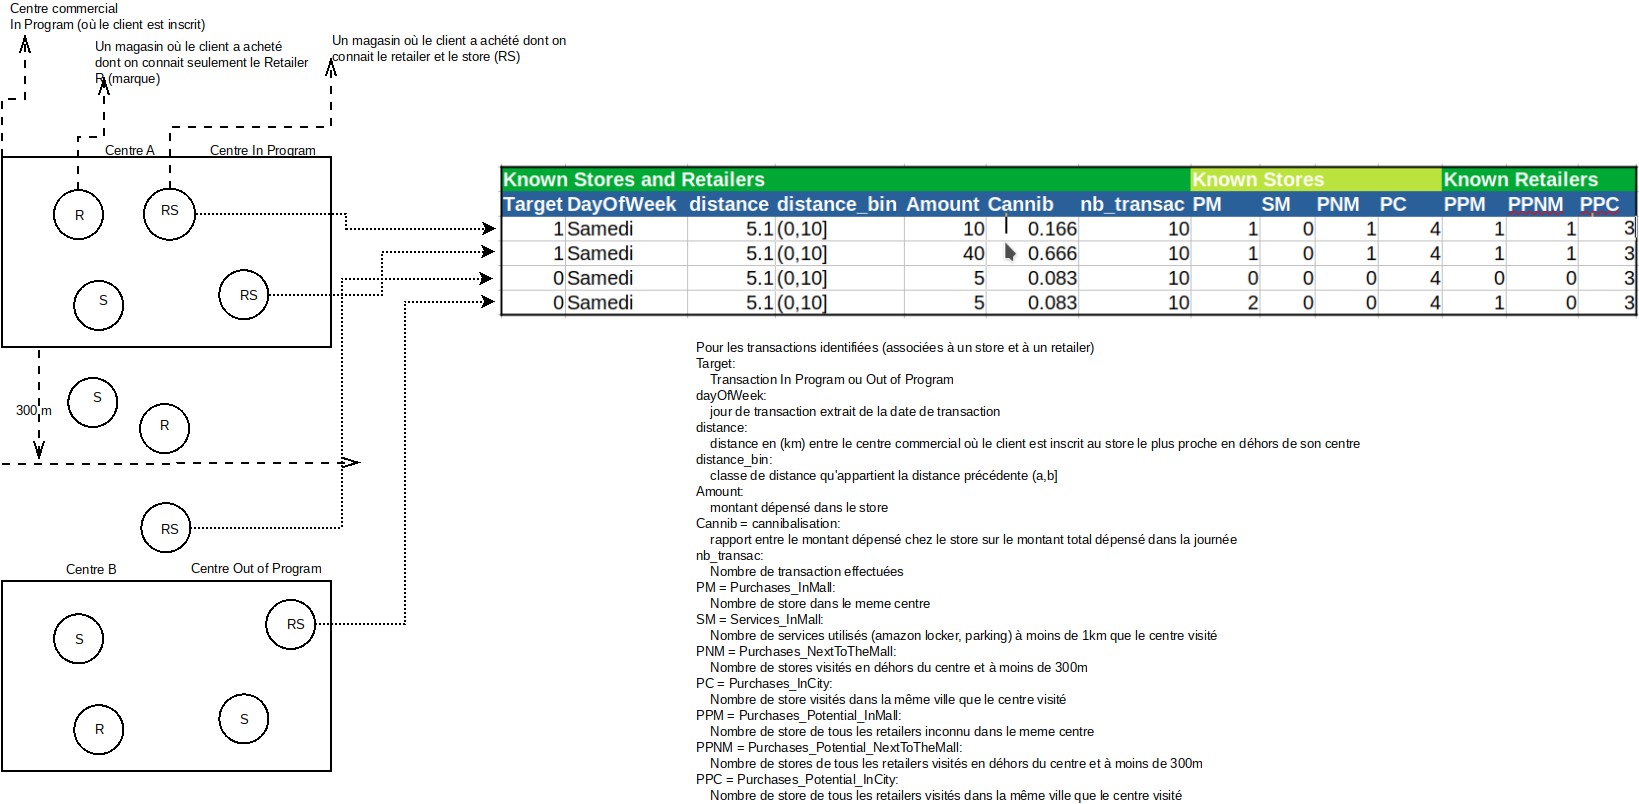
\includegraphics[width=15cm,height=8cm]{images/feature_engineering.png}
\caption[Systeme de calcule des variables]{Systeme de calcule des variables}
\label{monlabel}
\end{center}
\end{figure}


Dans le schéma ci-dessous on peut remarquer deux centres commerciaux (Centre A et Centre B) à gauche. Le centre A est le centre commercial où le client est inscrit, en d’autre terme le centre A est “In program”. Les petits cercles sont les magasins visités par un client dans la même journée: quatre magasins dans le centre In program dont deux sont identifiables (R: détaillant, S: magasin) et deux autres dont on connaît seulement respectivement le détaillant (R) et le magasin (S). Tous les autres magasins dans le centre B et à l’extérieur sont considérés comme “out of program”.\\

La dataset entrant dans l’apprentissage de notre modèle est construite en appliquant le scoring sur les transactions effectuées dans la même journée dont le détaillant et le magasin sont identifiables. \\

On charge seulement les transactions des clients qui sont inscrits dans
un programme (centre commercial) donné ex: Les 4 Temps, Okabe,...



\begin{itemize}
\item Target: \\
Une transaction est in-programme si la transaction est effectuée dans un magasin du centre où le client est inscrit.
\item distance: \\
Calculer la distance entre le centre où le client est inscrit 
aux autres magasins qu'il a aussi visité et considérer celui qui est proche du centre.
\item distance-bin: \\
Classer la distance du magasin le plus proche dans une classe de distance €(a,b]
\item DayOfWeek:\\ 
Jour de la transaction extrait de la date de la transaction.
\item Amount:\\
Montant dépensé dans le magasin
\item Cannibalisation:\\
Poids du détaillant dans le centre: Rapport entre le montant dépensé par les clients chez le détaillant sur le montant total dépensé dans le centre sur une période.
\item Nb-transaction:\\
Quantité totale d'articles achetés par le client dans la même journée.
\item ServicesInMall:\\
Nombre de services utilisés par le client dans la journée (amazon locker, parking) à moins de un kilomètre du centre commercial
\item Purchases-InMall:\\
Nombre de magasin visité dans le centre dans la journée
\item Purchases-NextToTheMall:\\
Nombre de magasins visités en dehors du centre et à moins de 300 mètres.
\item Purchases-InCity:\\
Nombre de magasins visités dans la même ville que le centre visité.
\item Purchases-Potential-InMall:\\
Nombre de magasins de tous les détaillants non identifiés que le client a visité dans le centre.
\item Purchases-Potential-NextToTheMall:\\
Nombre de magasins de tous les détaillants que le client a visité en dehors du centre et à moins de 300 mètres.
\item Purchases-Potential-InCity:\\
Nombre de magasins de tous les détaillants non identifiés visités dans la même ville que le centre.
\end{itemize}

Le calcul de ces variables étant coûteux en temps d'exécution, dans mon travail il a fallu migrer toutes les requêtes de calcul Postgres et certaines opérations dataframes Pandas vers Amazon Redshift.

\newpage
\section{Présentation des données}
\subsection{Dataset:}
Après calcul sur l'ensemble des transactions en base le jeu de données comporte 483725 lignes sur 14 variables.
\begin{figure}[h]
\begin{center}
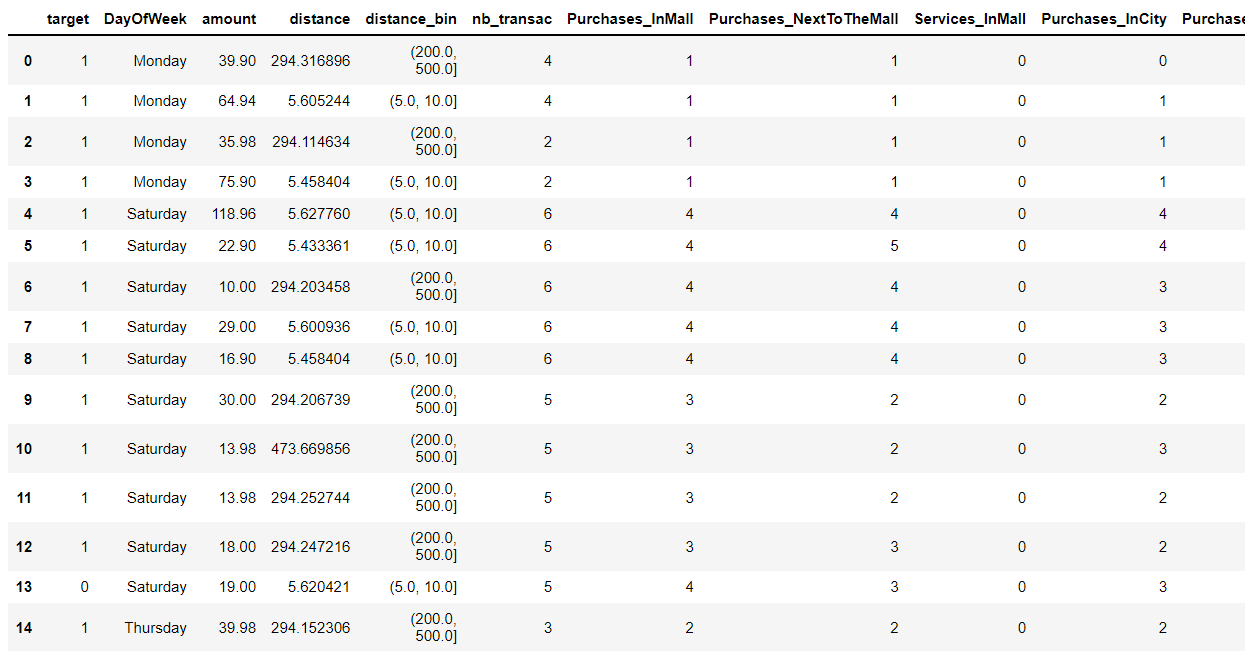
\includegraphics[width=15cm,height=6cm]{images/dataset_1.png}
\caption[Jeu de donnée]{Jeu de donnée}
\label{monlabel}
\end{center}
\end{figure}

\begin{figure}[h]
\begin{center}
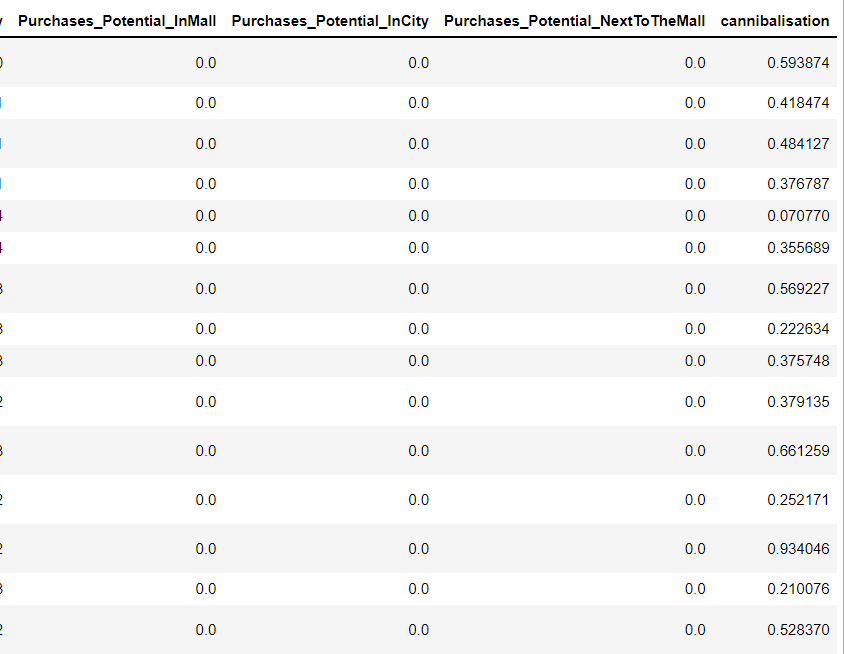
\includegraphics[width=15cm,height=6cm]{images/dataset_2.png}
\caption[Jeu de donnée]{Jeu de donnée}
\label{monlabel}
\end{center}
\end{figure}







